% !TEX TS-program = xepythontex

\documentclass[10pt, envcountsect , spanish]{beamer}


\newif\ifnotas
\notasfalse% Para no mostrar los globos
\notastrue % Para  mostrar los globos

\input ../preambulo.tex

\usepackage[normalem]{ulem}               % to striketrhourhg text
\newcommand\tacha{\bgroup\markoverwith{\textcolor{black}{\rule[0.5ex]{2pt}{0.8pt}}}\ULon}






%································ TITULO, AUTOR, ETC

\title[Interfaces]{Clases Abstractas, interfaces}
\subtitle{Polimorfirmo}

\author[L. Daniel Hernández]{L. Daniel Hernández $<ldaniel@um.es>$}

\institute[ldaniel@um.es]{Dpto. Ingeniería de la Información  y las Comunicaciones\\ Universidad de Murcia \\ 14 de noviembre de 2023\newline \hrule}


\date[ldaniel@um.es]{ 
\vskip 1.0cm
%\vskip -1.25cm
%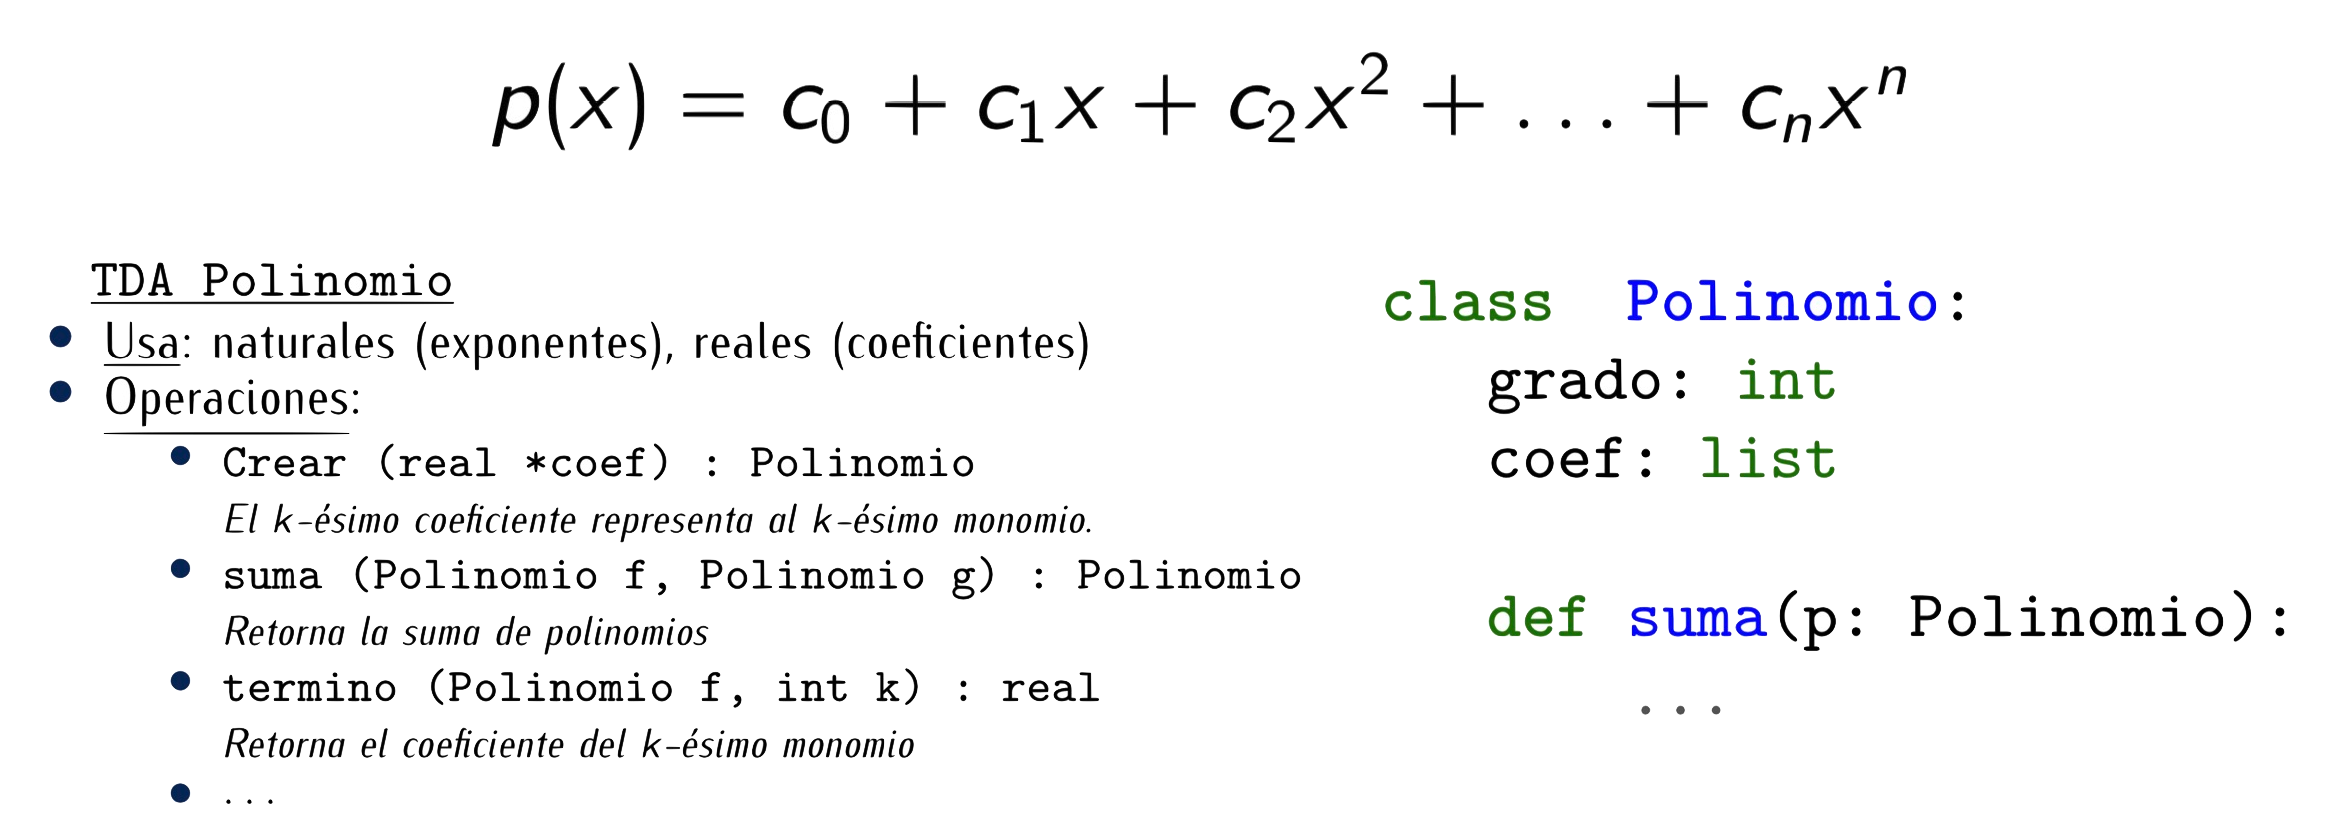
\includegraphics[width=.8\textwidth, height=.18\textheight]{fig/polinomio}
}

\graphicspath{{img/}}






%%%%%%%%%%%%%%%%%%%%%%%%%%%%%%%%%%
%%%%%%%%%%%%%%%%%%%%%%%%%%%%%%%%%%
%%%%%%%%%%%%%%%%%%%%%%%%%%%%%%%%%%
%%%%%%%%%%%%%%%%%%%%%%%%%%%%%%%%%%

%https://es.overleaf.com/learn/how-to/Writing_Markdown_in_LaTeX_Documents
\usepackage[hashEnumerators]{markdown}


%%%%%%%%%%%%%%%%%%%%%%%%%%%%%%%%%%
%%%%%%%%%%%%%%%%%%%%%%%%%%%%%%%%%%
%%%%%%%%%%%%%%%%%%%%%%%%%%%%%%%%%%
%%%%%%%%%%%%%%%%%%%%%%%%%%%%%%%%%%
\begin{document}

%\pgfdeclareimage[height=1cm]{logo}{logo.png}
%\logo{\pgfuseimage{logo}}



%--------------------------------------------------------------------------------
{\usebackgroundtemplate{%
  \includegraphics[width=\paperwidth,height=\paperheight]{../img/fondoUMUCompleto}}

\begin{frame}[b]
	\maketitle

\begin{tikzpicture}[overlay, remember picture]
\node[anchor=south west, %anchor is bottom left corner of the graphic
      xshift=.43\textwidth, %shifting around
      yshift=0.7cm] 
     at (current page.south west) %left bottom corner of the page
     {\includegraphics[width=.4\textwidth, height=.3\textheight]{fig/polimorfismo}
     \footnote[frame]{\tiny
Imagen: Codejavu }}; 
\end{tikzpicture}
	
\end{frame}			% Transparencia: Título
}



%
%
%
%%%cajero.png   https://www.freepik.es/vector-gratis/elementos-cajero-automatico_959486.htm}}}
%%\mail{ivan dot valbusa at univr dot it}
%\institute[DIIC. Univ. de Murcia] % (optional)
%{
%  Departamento de Ingeniería de la Información y las Comunicaciones\\
%  Universidad de Murcia
%}
%\date{\today\ (\currenttime h)}
%\titlegraphic[width=.45\textwidth]{fig/polimorfismo}{xshift=-1.0cm, yshift=-.05\textheight}





%%%%%%%%%%%%%%%%%%%%%%%%%%%%%%%%%%%%%%%%%%%%%%%%
%%%%%%%%%%%%%%%%%%%%%%%%%%%%%%%%%%%%%%%%%%%%%%%%
\begin{frame}{Índice de Contenidos}\tableofcontents \end{frame}



%%%%%%%%%%%%%%%%%%%%%%%%%%%%%%%%%%%%%
%%%%%%%%%%%%%%%  SECTION   %%%%%%%%%%%%%%%
%%%%%%%%%%%%%%%%%%%%%%%%%%%%%%%%%%%%%
\section{Clases Abstractas}




%%%%%%%%%%%%%%%%%%%%%%%%%%%%%%%%%%%%%
%%%%%%%%%%%%%%%%%%%%%%%%%%%%%%%%%%%%%
\begin{frame}{Clases Abstractas} 

\begin{itemize}
\item La \key{abstracción} es el proceso por el que captamos las características esenciales de un objeto tanto en atributos como en comportamiento.

\item \textbf{Las clases abstractas codifican altos niveles de abstracción}

\item Una \key[red]{clase abstracta representa} a objetos para los que \key{conocemos algunas de las variables} que definen su estado y \key{conocemos algunas de sus funcionalidades} \key[red!50!yellow]{pero no sabemos establecerlas} sin concretar el objeto.

\item Un \key{método abstracto} es aquel que tiene declaración pero no está  definido.


\item Una \key{clase abstracta} es la que tiene (al menos) un método abstracto

\item 
\fbox{\begin{minipage}{.9\textwidth}
Una clase abstracta es una clase que (1) \textbf{no se puede instanciar} (no representan algo específico), (2) \textbf{se usa únicamente para definir subclases}
\end{minipage}}



\item Una \key{subclase puede ser abstracta} si la clase padre lo es.


\item Existirán \key{subclases} de una clase abstracta  que \key{implementarán} los métodos abstractos.

\item Por tanto, tendremos \key{un método} (abstracto) que \key{se ejecutará de forma diferente} en cada subclase:
\key[red]{Polimorfismo de inclusión o subtipado}.


\item Una clase abstracta puede tener constructores:
\begin{itemize}
\item Pero no sirven para construir instancias (por definición de clase abstracta).
\item Las subclases no abstractas deberá de sobreescribir el constructor \key{explícito} con los mismos parámetros  y deben llamar al constructor del padre (abstracto) con \cm{super()}.
\end{itemize}

\end{itemize}

\end{frame}
% . . . . . . . . . . . . . . . . . . . . . . . . . . . . . . . . . . . . . . . . . . . . . . . . . . . . . . 
% . . . . . . . . . . . . . . . . . . . . . . . . . . . . . . . . . . . . . . . . . . . . . . . . . . . . . . 



%%%%%%%%%%%%%%%%%%%%%%%%%%%%%%%%%%%%%
%%%%%%%%%%%%%%%%%%%%%%%%%%%%%%%%%%%%%
\begin{frame}[fragile]{Ejemplo de Clase Abstracta} 

\unEjemplo
\begin{itemize}
\item La clase \key[magenta]{Animal} tiene los métodos \cm{caminar()} o \cm{comer()} pero no se sabe cuáles son las acciones concretas que deben realizarse.
\item Por tanto, la clase \key[magenta]{Animal}  \textbf{debe de ser} \key{abstracta}.
\item Las clase \key[magenta]{Ave} y \key[magenta]{Mamífero} son subclases de Animal.
\item \key[magenta]{Ave} y \key[magenta]{Mamífero} heredan el método \cm{caminar()} que lo harán de forma diferente, 
\begin{itemize}
\item Una \key[magenta]{ave} camina con \textbf{dos} patas pero un \key[magenta]{mamífero} camina con \textbf{cuatro} patas.
\end{itemize}
\end{itemize}

\footnotesize
\begin{columns}
\begin{column}{.45\textwidth}
\begin{pyconsole}[][frame=single, fontsize=\scriptsize]
from abc import ABC, \
        abstractmethod
class Animal(ABC):
  @abstractmethod
  def caminar(self):
    pass
    
class Mamifero(Animal):
  def caminar(self):
    print("... con 4 patas")
    
class Ave(Animal):
  pass

 \end{pyconsole}
\end{column}
\begin{column}{.54\textwidth}  
\begin{pyconsole}[][frame=single, fontsize=\scriptsize] 
perro = Mamifero()
perro.caminar()
gallo = Ave()
\end{pyconsole}

\normalsize
Si una clase hija \key{no} define el método abstracto sigue siendo una clase abstracta.

\end{column}
\end{columns}

\end{frame}
% . . . . . . . . . . . . . . . . . . . . . . . . . . . . . . . . . . . . . . . . . . . . . . . . . . . . . . 
% . . . . . . . . . . . . . . . . . . . . . . . . . . . . . . . . . . . . . . . . . . . . . . . . . . . . . . 




%%%%%%%%%%%%%%%%%%%%%%%%%%%%%%%%%%%%%
%%%%%%%%%%%%%%%  SECTION   %%%%%%%%%%%%%%%
%%%%%%%%%%%%%%%%%%%%%%%%%%%%%%%%%%%%%
\section{Interfaces}

%%%%%%%%%%%%%%%%%%%%%%%%%%%%%%%%%%%%%
%%%%%%%%%%%%%%%%%%%%%%%%%%%%%%%%%%%%%
\begin{frame}{Interfaces} 

\begin{itemize}
\item 
Una \key{interfaz} es una abstracción \textbf{basada solo} en la funcionalidad y definen un \key[red]{tipo}.


\item
Es solo un conjunto de \key{métodos}. NO tienen atributos de instancia.

\item
Son métodos \key{necesarios} en algunos objetos para que cumplan sus \key[red]{requisitos mínimos de  funcionalidad}.

\item 
Dichos objetos son del \key[red]{tipo} que diga el nombre de la interface (\key{subtipado estructural}). 

\item \key[red]{Polimorfismo de subtipado}: Añaden \key{especialización}/extensión a los objetos.

	\item 
	Cada objeto implementan la especialización de forma diferente:
		\begin{itemize} \small
		\item \key{Son métodos abstractos y polimórficos}
		\end{itemize}
		
	
\end{itemize}

\vfill

\hrule

\vfill

\centerline{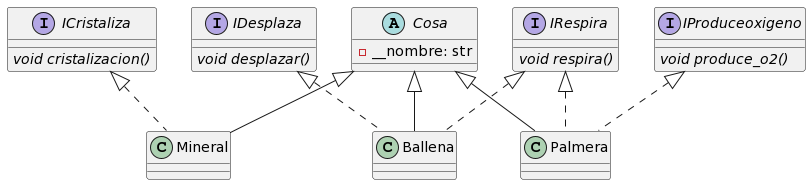
\includegraphics[width=.8\textwidth]{fig/mundoCosa}}

\small

En el mundo de la Cosa solo se conoce el nombre de las cosas.
Se tienen las siguientes subclases directas: mineral, ballena y palmera.
a sus objetos, se quieren dotar de las funcionalidades: cristaliza, desplaza, respira y produce oxígeno.
\end{frame}
% . . . . . . . . . . . . . . . . . . . . . . . . . . . . . . . . . . . . . . . . . . . . . . . . . . . . . . 
% . . . . . . . . . . . . . . . . . . . . . . . . . . . . . . . . . . . . . . . . . . . . . . . . . . . . . . 



%%%%%%%%%%%%%%%%%%%%%%%%%%%%%%%%%%%%%
%%%%%%%%%%%%%%%%%%%%%%%%%%%%%%%%%%%%%
\begin{frame}{Interfaces en Python} 

\begin{itemize}
\item \key[red]{Python} sigue la premisa \textbf{``Duck Typing''}.

\item Para \key[red]{Python} todo los objetos que tengan ciertos métodos definen un tipo de objetos.

\unEjemplo Todo lo que implemente \pyv{__iter__()} y \pyv{__next__()} es un iterador.


\item En \key[red]{Python} una clase debe \key{definir todos} los métodos requeridos para que se reconozca ``como un pato'' (un objeto de la interface).

\item En \key[red]{Python} \key{se debe  registrar una interface} para que cualquier objeto que implemente los métodos \textbf{sea reconocido} como objeto  del  tipo de la interface.

\item Se distinguen
\begin{itemize}
\item \key{Interfaces Informales}: 

\hfil Aquellas que \textbf{no} fuerzan a la sobreescritura de todos los métodos.


\item \key{Interfaces Formales}:  

\hfil Aquellas que \textbf{sí} fuerzan a la sobreescritura de todos los métodos.
\end{itemize}

\end{itemize}

\end{frame}
% . . . . . . . . . . . . . . . . . . . . . . . . . . . . . . . . . . . . . . . . . . . . . . . . . . . . . . 
% . . . . . . . . . . . . . . . . . . . . . . . . . . . . . . . . . . . . . . . . . . . . . . . . . . . . . . 


%%%%%%%%%%%%%%%%%%%%%%%%%%%%%%%%%%%%%
%%%%%%%%%%%%%%%%%%%%%%%%%%%%%%%%%%%%%
\begin{frame}[fragile]{Registro de una Interfaces en Python} 

\begin{itemize}
\item 
\key[red]{Python} es demasiado versátil para trabajar con registros de interfaces.
Puede consultar p.e. \url{https://realpython.com/python-interface/}

\item 
Una forma ``sencilla'' es sobreescribir el métodode clase  \key[blue]{\_\_subclasshook\_\_()}.

Se requiere el paquete \cm{abc} (Abstract Base Classes).


\footnotesize
\begin{pyconsole}[][frame=single]
import abc

class Interface(metaclass=abc.ABCMeta): # Es mejor poner abc.ABC
    """Esta es la interface usada. Se registra
   definiendo __subclasshook__ (con todos los métodos)
    """
    @classmethod
    def __subclasshook__(cls, subclass): # Aquí añade los métodos
        if cls is Interface:
            return (hasattr(subclass, 'metodo1') and
                    callable(subclass.metodo1) and
                    hasattr(subclass, 'metodo2') and
                    callable(subclass.metodo2))
        return NotImplemented

\end{pyconsole}

\item Lectura: Si la subclase tiene el atributo \textcolor{red!70!black}{\tt metodo1} y se puede invocar y  tiene el atributo \textcolor{red!70!black}{\tt metodo2} y se puede invocar, entonces es \textcolor{red!70!black}{\tt True} que es de la clase \textcolor{blue}{\tt IMovimiento}
\end{itemize}
\end{frame}
% . . . . . . . . . . . . . . . . . . . . . . . . . . . . . . . . . . . . . . . . . . . . . . . . . . . . . . 
% . . . . . . . . . . . . . . . . . . . . . . . . . . . . . . . . . . . . . . . . . . . . . . . . . . . . . . 







%%%%%%%%%%%%%%%%%%%%%%%%%%%%%%%%%%%%%
%%%%%%%%%%%%%%%%%%%%%%%%%%%%%%%%%%%%%
\begin{frame}[fragile]{Crear Interfaces Informales en Python} 

\begin{enumerate}

\item[1.] Crear el registro del interface con la siguiente sintaxis:

\footnotesize
\begin{pyconsole}[][frame=single, fontsize=\scriptsize]
import abc

class IMovible(metaclass=abc.ABCMeta):
    """Esta es la interface usada. Se registra
   definiendo __subclasshook__ (con todos los métodos)
    """
    @classmethod
    def __subclasshook__(cls, subclass): # Aquí añade los métodos
        if cls is IMovible:
            return (hasattr(subclass, 'movimiento') and
                    callable(subclass.movimiento) and
                    hasattr(subclass, 'lo_que_mueve') and
                    callable(subclass.lo_que_mueve))
        return NotImplemented

\end{pyconsole}

\normalsize

\item[2.] Crear las clases que quieran implementar la interface

\footnotesize
\begin{pyconsole}[][frame=single, fontsize=\scriptsize]
class Vaca:
    def movimiento(self):
        print("Se desplaza a 4 patas")
    def lo_que_mueve(self):
        print("Muevo la cola")

\end{pyconsole}
\end{enumerate}

\end{frame}
% . . . . . . . . . . . . . . . . . . . . . . . . . . . . . . . . . . . . . . . . . . . . . . . . . . . . . . 
% . . . . . . . . . . . . . . . . . . . . . . . . . . . . . . . . . . . . . . . . . . . . . . . . . . . . . . 



%%%%%%%%%%%%%%%%%%%%%%%%%%%%%%%%%%%%%
%%%%%%%%%%%%%%%%%%%%%%%%%%%%%%%%%%%%%
\begin{frame}[fragile]{Ejemplo de Interfaces Informales en Python} 
\begin{itemize}

\item Solo los objetos de las clases que implementen la interfaces serán reconocidos como instancias de la interface.

\

\scriptsize
\begin{pyconsole}[][frame=single, fontsize=\scriptsize]
class Vaca:
    def movimiento(self):
        print("Se desplaza a 4 patas")
    def lo_que_mueve(self):
        print("Muevo la cola")

v = Vaca(); isinstance(v, IMovible)  # El objeto es de su clase
issubclass(Vaca, IMovible) # Están los dos métodos 

class Serpiente:
    def movimiento(self):
        print("Repto como una serpiente")   
                 
s = Serpiente(); isinstance(s, IMovible) # Falta el método queMueve()
issubclass(Serpiente, IMovible) # Falta el método queMueve()
\end{pyconsole}


Observa que en \pyv{Vaca} no se ha indicado ningún tipo de herencia sobre \pyv{IMovimiento} para que Python la reconozca como una  subclase.
\end{itemize}

\end{frame}
% . . . . . . . . . . . . . . . . . . . . . . . . . . . . . . . . . . . . . . . . . . . . . . . . . . . . . . 
% . . . . . . . . . . . . . . . . . . . . . . . . . . . . . . . . . . . . . . . . . . . . . . . . . . . . . . 




%%%%%%%%%%%%%%%%%%%%%%%%%%%%%%%%%%%%%
%%%%%%%%%%%%%%%%%%%%%%%%%%%%%%%%%%%%%
\begin{frame}[fragile]{Creación de Interfaces Formales en Python - I} 

\begin{enumerate}

\item[1.] \small Crear el registro de la interface y \key{añadir} los métodos como \key{métodos abstractos} con la siguiente sintaxis:

\footnotesize
\begin{pyconsole}[][frame=single, fontsize=\scriptsize]
import abc

class IMovible(abc.ABC):
    """Esta es la interface.
    Es necesario definir __subclasshook__ con todos los métodos abstractos.
    """
    @classmethod
    def __subclasshook__(cls, subclass):
        if cls is IMovible:
            return (hasattr(subclass, 'movimiento') and
                    callable(subclass.movimiento) and
                    hasattr(subclass, 'lo_que_mueve') and
                    callable(subclass.lo_que_mueve))
        return NotImplemented   
    @abc.abstractmethod
    def movimiento(self):  # Esto lo diferencia de las informales
        pass  
    @abc.abstractmethod
    def lo_que_mueve(self):
        pass
        
\end{pyconsole}

\end{enumerate}

\end{frame}
% . . . . . . . . . . . . . . . . . . . . . . . . . . . . . . . . . . . . . . . . . . . . . . . . . . . . . . 
% . . . . . . . . . . . . . . . . . . . . . . . . . . . . . . . . . . . . . . . . . . . . . . . . . . . . . . 



%%%%%%%%%%%%%%%%%%%%%%%%%%%%%%%%%%%%%
%%%%%%%%%%%%%%%%%%%%%%%%%%%%%%%%%%%%%
\begin{frame}[fragile]{Interfaces Formales en Python - II} 
\begin{enumerate}

\item[2.] Parar \key{forzar} su  implementación deberá \key{indicar que la interface es una superclase}.

\scriptsize
\begin{pyconsole}[][frame=single, fontsize=\scriptsize]
class Vaca:     # Esta clase, si quiere no implementa la interface
    def movimiento(self):
        print("Se desplaza a 4 patas")
    def lo_que_mueve(self):
        print("Muevo la cola")


class Serpiente(IMovible):  # Esta clase está forzada a implementar la interface
    def movimiento(self):
        print("Repto como una serpiente")

v = Vaca();
print(isinstance(v, IMovible))  # El objeto es de su clase
print(issubclass(Vaca, IMovible)) # Están los dos métodos


s = Serpiente(); # Falta el método lo_que_mueve()
\end{pyconsole}
\end{enumerate}

\scriptsize

Observa que en \pyv{Vaca} no se ha indicado ningún tipo de herencia sobre \pyv{IMovimiento} para que Python la reconozca como una  subclase (definición informal).

\end{frame}
% . . . . . . . . . . . . . . . . . . . . . . . . . . . . . . . . . . . . . . . . . . . . . . . . . . . . . . 
% . . . . . . . . . . . . . . . . . . . . . . . . . . . . . . . . . . . . . . . . . . . . . . . . . . . . . . 



%%%%%%%%%%%%%%%%%%%%%%%%%%%%%%%%%%%%%
%%%%%%%%%%%%%%%  SECTION   %%%%%%%%%%%%%%%
%%%%%%%%%%%%%%%%%%%%%%%%%%%%%%%%%%%%%
\section{Mixin}

%%%%%%%%%%%%%%%%%%%%%%%%%%%%%%%%%%%%%
%%%%%%%%%%%%%%%%%%%%%%%%%%%%%%%%%%%%%
\begin{frame}{Mixin (Mezclas)} 

\begin{itemize}
\item  Un \key{mixin} no es ni una clase abstracta ni una interface.

\item  Es una clase que 
	\begin{itemize}
	\item \key{Añade funcionalidad} a otras clases
	\begin{itemize}
	\item Permite a un programador \key{inyectar código} en las clases que lo necesiten.
	\end{itemize}
	
	
	\item \key{No añade especialización}

	\begin{itemize}
	\item Los métodos inyectados en la clase no se pueden considerar como una especialización  de la clase.
	\end{itemize}
	
	\item \key{No tiene sentido} que tengan  objetos o  clases derivadas.
	
	\begin{itemize}
	\item El mixin no se considera una clase base.
	\end{itemize}
	
	\end{itemize}

{\footnotesize

}

\end{itemize}

\begin{columns}

\begin{column}{.78\textwidth}

\begin{itemize}

\item Se usa siempre de la siguiente manera: \\
\hfil \key{la clase B extiende (A con Mixin)}

\item \key{Conceptualmente} \textbf{es como si} se creara la clase  \textbf{A-con-M} donde
\begin{itemize}
\item La clase padre de \textbf{A-con-M} es \textbf{A}
\item La clase padre de \textbf{B} es \textbf{A-con-M}
\end{itemize}

\item Ejemplos que hay que conocer: \href{https://docs.python.org/3/library/collections.abc.html}{collections.abc — Abstract Base Classes for Containers¶}

\end{itemize}
\end{column}

\begin{column}{.2\textwidth}
\centerline{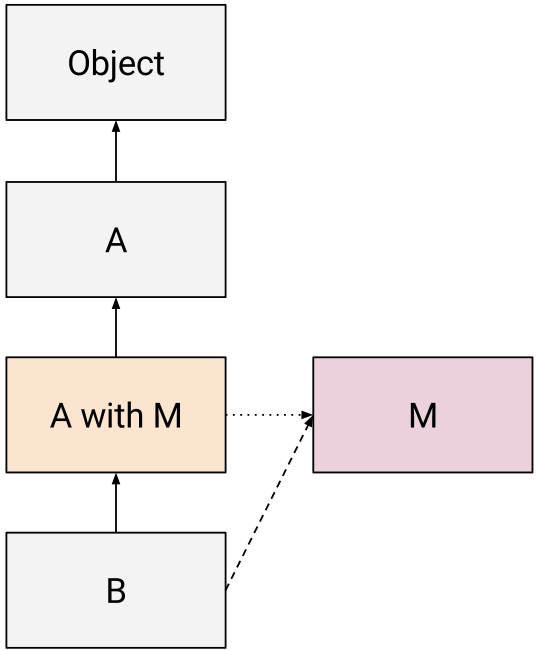
\includegraphics[width=\textwidth]{fig/class-hierarchy-2}}
\end{column}

\end{columns}
\end{frame}
% . . . . . . . . . . . . . . . . . . . . . . . . . . . . . . . . . . . . . . . . . . . . . . . . . . . . . . 
% . . . . . . . . . . . . . . . . . . . . . . . . . . . . . . . . . . . . . . . . . . . . . . . . . . . . . . 





%%%%%%%%%%%%%%%%%%%%%%%%%%%%%%%%%%%%%
%%%%%%%%%%%%%%%%%%%%%%%%%%%%%%%%%%%%%
\begin{frame}[fragile]{Ejemplo de Mixin en Python}{\url{https://programmerclick.com/article/8047526022/}}

\begin{itemize}
\item En \key[red]{Python} los \key{Mixins} se crean con \key{herencia múltiple}
\end{itemize}

\footnotesize
\begin{pyverbatim}[][frame=single, fontsize=\scriptsize]
class Displayer():
    def display(self, message):
        print(message)

# Este Mixin añade la funcionalidad de Mostrar + Registrar
# Para Mostrar se delega en el padre.
# Este Mixin solo lo pueden usar las clases cuyo padre tengan display()    
class LoggerMixin():
    def log(self, message, filename='logfile.txt'):
        with open(filename, 'a') as fh:
            fh.write(message)
    def display(self, message):
        super().display(message) # << No todos los objetos lo tienen
        self.log(message)

class MySubClass(LoggerMixin, Displayer):
    def log(self, message):
        super().log(message, filename='subclasslog.txt')

subclass = MySubClass()
subclass.display("This string will be shown and logged in subclasslog.txt")
\end{pyverbatim}

\end{frame}
% . . . . . . . . . . . . . . . . . . . . . . . . . . . . . . . . . . . . . . . . . . . . . . . . . . . . . . 
% . . . . . . . . . . . . . . . . . . . . . . . . . . . . . . . . . . . . . . . . . . . . . . . . . . . . . . 







%%%%%%%%%%%%%%%%%%%%%%%%%%%%%%%%%%%%%
%%%%%%%%%%%%%%%  SECTION   %%%%%%%%%%%%%%%
%%%%%%%%%%%%%%%%%%%%%%%%%%%%%%%%%%%%%
\section{Clases Abstractas vs Interfaces vs Mixin}




%%%%%%%%%%%%%%%%%%%%%%%%%%%%%%%%%%%%%
%%%%%%%%%%%%%%%%%%%%%%%%%%%%%%%%%%%%%
\begin{frame}{Intefaces vs Clases Abstractas vs Mixin - I}
{\tiny \url{https://codesitio.com/recursos-utiles-para-tu-web-o-blog/cursos/curso-de-java-clases-abstractas-e-interfaces/}} %#Estructura_basica_de_un_interfaz

\Large

\begin{itemize}
\item Una \key[red]{clase abstracta} se caracteriza por:

\begin{itemize} \large
\item \textbf{Constructores}: Tiene al menos uno (el implícito)
\item \textbf{Variables de Clase}: Se admiten
\item \textbf{Campos}: Pueden tener cualquier modificador de visualización.
\item \textbf{Métodos estáticos}: Tendrán \key{signatura y cuerpo}. No pueden ser abstractos. 
\item \textbf{Métodos de instancia}: 
	\begin{itemize} \normalsize
	\item Pueden tener \key{signatura y cuerpo}. 
	\item \textbf{Al menos uno} tendrá el modificador \pyv{@abstractmethod}: Tendrá \key{signatura pero no cuerpo}
	\end{itemize}
	
\item \textbf{Sobreescritura de métodos:} está permitida

\item Los métodos pueden tener \key{cualquier modificador} de visualización.

\item \key{Admiten herencia}.

\hfil En esto casos se habla de subclase y de superclase.
\end{itemize}

\end{itemize}
\end{frame}
% . . . . . . . . . . . . . . . . . . . . . . . . . . . . . . . . . . . . . . . . . . . . . . . . . . . . . . 
% . . . . . . . . . . . . . . . . . . . . . . . . . . . . . . . . . . . . . . . . . . . . . . . . . . . . . . 




%%%%%%%%%%%%%%%%%%%%%%%%%%%%%%%%%%%%%
%%%%%%%%%%%%%%%%%%%%%%%%%%%%%%%%%%%%%
\begin{frame}{Intefaces vs Clases Abstractas vs Mixin - I}
{\tiny \url{https://codesitio.com/recursos-utiles-para-tu-web-o-blog/cursos/curso-de-java-clases-abstractas-e-interfaces/}} %#Estructura_basica_de_un_interfaz

\Large 

\begin{itemize}

\item Una \key[red]{interface} se caracteriza por:



\begin{itemize} \large
\item \textbf{Constructores}: NO tiene.

\item \textbf{Variables de Clase}: Se admiten

\item \textbf{Campos}: NO tiene. Algunos lenguajes relajan esto.


Es decir, no existen variables de objeto y son solo de clase.

\item \textbf{Métodos estáticos}: Tendrán \key{signatura y cuerpo}. 

\item \textbf{Métodos de instancia}: Contendrán \key{solo la signatura}, sin cuerpo. 

Tendrá el modificador \pyv{@abstractmethod} o sentencia similar.

\item \textbf{Sobreescritura de métodos:} \textbf{Todos} se deben  \key{sobreescribir}.

\item Todos los métodos (estáticos y de instancia) serán  \key{públicos}.


\item \key{Admiten herencia}.

\hfil En esto casos se habla de subinterface y de superinterface.

\end{itemize}

\end{itemize}
%https://es.ccm.net/contents/413-oop-polimorfismo

\end{frame}
% . . . . . . . . . . . . . . . . . . . . . . . . . . . . . . . . . . . . . . . . . . . . . . . . . . . . . . 
% . . . . . . . . . . . . . . . . . . . . . . . . . . . . . . . . . . . . . . . . . . . . . . . . . . . . . . 






%%%%%%%%%%%%%%%%%%%%%%%%%%%%%%%%%%%%%
%%%%%%%%%%%%%%%%%%%%%%%%%%%%%%%%%%%%%
\begin{frame}{Intefaces vs Clases Abstractas vs Mixin - II}

\Large 

\begin{itemize}

\item Una \key[red]{Mixin} se caracteriza por:
\begin{itemize} \large
\item \textbf{Constructores}: NO tiene.

\item \textbf{Variables de Clase}: Se admiten

\item \textbf{Campos}: Se admiten

\item \textbf{Métodos estáticos}: Tendrán \key{signatura y cuerpo}. 
\item \textbf{Métodos de instancia}: 
	\begin{itemize} \normalsize
	\item Deberían tener \key{signatura y cuerpo}. 
	\item Pero \textbf{se permite} que  tengan el modificador \pyv{@abstractmethod}.
	\end{itemize}

\item \textbf{Sobreescritura de métodos:} No se deberían de sobreescribir salvo que sean abstractos.

\item Todos los métodos (estáticos y de instancia) serán  \key{públicos}.

\item No son auténticas clases. No tiene sentido crear subclases del Mixin. Evitar  \pyv{@abstractmethod}.


\item Nota: serán heredados por las subclases de la clase Mezcla pero las subclases no deberían de modificarlos (no deberán crear especificidad en los métodos del Mixin)

\end{itemize}

\end{itemize}
%https://es.ccm.net/contents/413-oop-polimorfismo

\end{frame}
% . . . . . . . . . . . . . . . . . . . . . . . . . . . . . . . . . . . . . . . . . . . . . . . . . . . . . . 
% . . . . . . . . . . . . . . . . . . . . . . . . . . . . . . . . . . . . . . . . . . . . . . . . . . . . . . 




%%%%%%%%%%%%%%%%%%%%%%%%%%%%%%%%%%%%%
%%%%%%%%%%%%%%%%%%%%%%%%%%%%%%%%%%%%%
\begin{frame}{Intefaces vs Clases Abstractas vs Mixin - III}

\centering
\resizebox{\textwidth}{!}{%
\begin{tabularx}{\textwidth}{|l||X|X|X|} \hline
                       & C. Abstracta                & Interface        & Mixin                            \\ \hline
Constructor            & Sí                          & \textbf{No}               & \textbf{No}                               \\
Atributos de clase     & Sí                          & Sí               & Sí                               \\
Atributos de instancia & Sí                          & \textbf{No}               & Sí                               \\
Métodos estáticos      & Sí                          & Sí               & Sí                               \\
Métodos de clase       & Sí                          & Sí               & Sí                               \\
Métodos de instancia   & Sí. Al menos uno abstracto. & Todos abstractos & Sí. Alguno podría ser abstracto. \\
Sobreescritura         & Sí                          & Sí. Todos.       & \textbf{No} se debería.          \\
Herencia               & Sí                          & Sí               & \textbf{No}              \\ \hline               
\end{tabularx}%
}

\end{frame}
% . . . . . . . . . . . . . . . . . . . . . . . . . . . . . . . . . . . . . . . . . . . . . . . . . . . . . . 
% . . . . . . . . . . . . . . . . . . . . . . . . . . . . . . . . . . . . . . . . . . . . . . . . . . . . . . 







%%%%%%%%%%%%%%%%%%%%%%%%%%%%%%%%%%%%%
%%%%%%%%%%%%%%%  SECTION   %%%%%%%%%%%%%%%
%%%%%%%%%%%%%%%%%%%%%%%%%%%%%%%%%%%%%
\section{Tipos Genéricos}


%%%%%%%%%%%%%%%%%%%%%%%%%%%%%%%%%%%%%
%%%%%%%%%%%%%%%%%%%%%%%%%%%%%%%%%%%%%
\begin{frame}[fragile]{Tipos Genéricos: Introducción}  

\begin{itemize}
\item Considera el siguiente código para definir un objeto \; \cm{Entero}

{\small
\begin{pyverbatim}[][frame=single]
class Entero:
    self._valor: int
    def get(self) -> int:
        return self._valor
    def set(self, valor: int):
        self._valor = valor
\end{pyverbatim}
}

\item Si ahora queremos objetos con la misma funcionalidad para \cm{float}, \cm{str}, ... \textbf{habrá que repetir el código para cada uno de los tipos de datos}.

\item Una alternativa es utilizar el siguiente código a falta de indicar el tipo de dato \cm{<T>}

\begin{code}
class Tipo<T> {  // Clase paramétrica
  private T t;
  public  T   get()    { return t;   }
  public void set(T t) { this.t = t; }
}
\end{code}


\item Estaría genial poder generalizar esta idea con datos simples y estructuras de datos. 

P.e. Se podría reutilizar todo el código de cierta clase \cm{Lista} a falta de determinar el tipo de dato; es decir, utilizar \cm{Lista[T]} en vez de una para cada tipo de dato como \cm{ListaEntero}, \cm{ListaDouble}, ... .

\end{itemize}

\end{frame}
% . . . . . . . . . . . . . . . . . . . . . . . . . . . . . . . . . . . . . . . . . . . . . . . . . . . . . . 
% . . . . . . . . . . . . . . . . . . . . . . . . . . . . . . . . . . . . . . . . . . . . . . . . . . . . . . 




%%%%%%%%%%%%%%%%%%%%%%%%%%%%%%%%%%%%%
%%%%%%%%%%%%%%%%%%%%%%%%%%%%%%%%%%%%%
\begin{frame}[fragile]{Uso de  Tipos Genéricos en Python} 
\small
\begin{pyconsole}[][frame=single, fontsize=\scriptsize]
from typing import TypeVar, Generic # Definición de tipos
T = TypeVar('T')          # Definición de un tipo genérico
class Tipo(Generic[T]):  # Clase genérica
    _valor: T
    def get(self) -> T:
        return self._valor
    def set(self, valor: T):
        self._valor = valor

entero: Tipo[int] = Tipo[int]()  # Especifica el genérico como entero
entero.set(5)
entero.get()
# El tipado de Python es caprichoso
entero.set(5.6)   # Pero Python funciona por contrato !!!
entero.get()
\end{pyconsole}

\begin{itemize}
\item Los errores se mostrarán en el IDE siempre que declares el tipo antes del constructor, pero te dejará ejecutar el programa !!!
\end{itemize}
\end{frame}
% . . . . . . . . . . . . . . . . . . . . . . . . . . . . . . . . . . . . . . . . . . . . . . . . . . . . . . 
% . . . . . . . . . . . . . . . . . . . . . . . . . . . . . . . . . . . . . . . . . . . . . . . . . . . . . . 






%%%%%%%%%%%%%%%%%%%%%%%%%%%%%%%%%%%%%
%%%%%%%%%%%%%%%  SECTION   %%%%%%%%%%%%%%%
%%%%%%%%%%%%%%%%%%%%%%%%%%%%%%%%%%%%%
\section{Algunos Ejercicios}






%%%%%%%%%%%%%%%%%%%%%%%%%%%%%%%%%%%%%
%%%%%%%%%%%%%%%%%%%%%%%%%%%%%%%%%%%%%
\begin{frame}{Ejercicio} 
\small


\begin{ejercicio}{}
Los artefactos dispone de un motor capaz de indicar el número de revoluciones al que va.
Existen muchos tipos de motores cada uno con distintos tipos de atributos. ?Cómo modelar entonces la situación?
\end{ejercicio}


\setlist[itemize,1]{before*=\footnotesize, leftmargin=\dimexpr 7pt}%,label=$\triangleleft$}
\setlist[itemize,2]{before*=\footnotesize}%,label=\textbullet}


\begin{ejercicio}{}
\begin{itemize}\setlength{\itemsep}{0em}
\item La clase \key{SerieTV} tiene  el atributo número de episodios.
\item  La clase \key{VideoJuego} tiene  el atributo horas estimadas de juego.
\item Implementa para ambas clases su interface Getter/Setter.

\item Se considera ahora que ambas clases  pueden ser \cm{prestadas}.
?`qué se debería de hacer para que  tengan las siguientes acciones?

\begin{itemize} \setlength{\itemsep}{0em}
\item entregar(): cambia el atributo prestado a true.
\item devolver(): cambia el atributo prestado a false.
\item esEntregado(): devuelve el estado del atributo prestado.
\end{itemize}

\item Se considera ahora que  comparables: Si dos videojuegos tienen el mismo número de horas estimadas se consideran que son iguales.
Si dos series de tv tienen el mismo número de episodios se consideran que son iguales.

Ten en cuenta que pueden existir otros tipos de ocio que no pueden ser prestados, como los canales de streaming, pero si pueden ser comparables, por ejemplo, por el precio.
\end{itemize}

\end{ejercicio}

\end{frame}
% . . . . . . . . . . . . . . . . . . . . . . . . . . . . . . . . . . . . . . . . . . . . . . . . . . . . . . 
% . . . . . . . . . . . . . . . . . . . . . . . . . . . . . . . . . . . . . . . . . . . . . . . . . . . . . . 



%%%%%%%%%%%%%%%%%%%%%%%%%%%%%%%%%%%%%
%%%%%%%%%%%%%%%%%%%%%%%%%%%%%%%%%%%%%
\begin{frame}{Ejercicio} 
\footnotesize



\begin{ejercicio}{} Modela la siguiente situación y dibuja el diagrama UML asociado.

Un taller de carpintería tiene diferentes tipos de herramientas que conforme se van rompiendo se van añadiendo herramientas nuevas. Todas las herramientas tienen un uso que es diferente dependiendo de su objetivo. Se distinguen las herramientas universales y las herramientas específicas. Las universales constan de un conjunto de componentes que se pueden ir cambiando. Un ejemplo son las navajas suizas. Por otro lado las herramientas específicas se catalogan con un tipo basado en las tareas en las que pueda ser usado. Entre las específicas se distinguen la sierra circular que admite cierta potencia eléctrica y la lijadora que debe usarse a cierta velocidad de forma manual y cuya cuchilla se puede cambiar. Todas las herramientas eléctricas se pueden encender o apagar. 

% //www.plantuml.com/plantuml/png/ZPD1Rjim44NtFCKWgwI5SW0Z25Au1Rgmkt6oBhwfYJe6HGf3oeisxOswwX5oiJAi1KkA47Hd_ld_UVXDtyK4JNthJ9Bac3uA6aKBUjXkg6Poe1XSR-NvZyzdHtnWjM8bb5E2SwmlHWljn2VMvzymnZh4IFTbkXuc0lfXY2fo4XC-iofQOPyGLxJ9qir8kit6zuH6kO6EzCjlvyyh6WskIe2TjEB_D_7J6EnZKjX4PUFHUDZLXtQllA9TKl5D-P8-GY-lLdGCKh_D-1Gxjl8eTg0bwSA4rN2wprh63Me6lk8yU3coHhY2-VMlmAysj5tmUSxndFg28mxOzV8TsNpMT_A2MulQta5FwtGXiRU25ObFPHyRD46tg5bnlkC0sSW1TL1iuNku4-J8BbYfKPyfJWvBaF8A7c5vqf5ZcxHKLBBiBVkS7895H8S6kinQezqBz8Er78DAE75iaIUPnKQhwkbsl8zP_lrkdgfgOfiLMZ2BqRdp-ZexbmemithVGCwS1JdlOVcwozRngwcgMrgA6lFw_nmgkdXtCUdbZdtTj-ul

\end{ejercicio}



\begin{ejercicio}{} Modela la siguiente situación y dibuja el diagrama UML asociado.

Un zoológico tiene diferentes tipos de animales. Todos los animales tienen un nombre con un número de identificación. Todo carnívoros tienen una dieta especial diferente. Los hay que cazan y los que no. De entre los que cazan están los que son capaces de nadar, como el tigre, y los que no, como el león. También hay carnívoros cazadores que vuelan como el halcón peregrino. De entre los que no cazan está los carroñeros como los buitres.  También hay animales herbívoros, como los loros, capaces de volar, los hipopótamos, capaces de nadar, y las cebras


% //www.plantuml.com/plantuml/png/TP6zJiD03CTtFuL7FfG-G8LGeGn5AYm81ZOdTrIMBkVASJgKyaWCY4VeYy4rfqG98fFry__3oYqQ8xMs3c1imUCTqqQf9dn-MAFps4RSYuJZzuOh0U1eNj-eydZ_8e4Ktm7n4dTfFZkV_mxiu6EaUoJNwoAvVtLBslUwYlPZ7L3Pc59bM0Lg6ho9N5CugGkCKfVgv_Xaod5pGkpcoD6ITU9SaiRZvqvKijknD-hDgUjL12-At06GkwuEHO4hhsNd7k4X562OknsklSGfJN1BwcIqo54gno-l0lsOLxSjctf8NxvZY4lLKxZYhMp5gFwxMlfI2I2TXhFPuJh_VaWv7UZU5xhE4O9yUoVC3mn3sGWlV7Hj7Nu0

\end{ejercicio}

\end{frame}






%%%%%%%%%%%%%%%%%%%%%%%%%%%%%%%%%%%%%
%%%%%%%%%%%%%%%%%%%%%%%%%%%%%%%%%%%%%
\begin{frame}{Ejercicio} 
\footnotesize


\begin{ejercicio}{} Modela la siguiente situación y dibuja el diagrama UML asociado.

Cada recurso particular tiene un nombre y un precio; pero no se pueden construir instancias de esta clase. Los recursos forman grupos (el de los coches, el de la carne, etc...) y de cada grupo se puede saber si es comestible o no, y cada uno tiene un IVA diferente. 
Un producto es capaz de calcular su precio  y obtener el precio final de una lista de productos.
Son recursos los coches (de los que sabe su velocidad), la carne (de lo que se sabe su origen) y el pan (se conoce sus calorías).   El nombre de cada coche, carne o pan coincide con el de la clase a la que pertenece. 
De todos ellos se puede calcular su precio.
De entre todos los objetos se pueden distinguir  los comestibles (de los que se sabe cómo se comen y el sonido que hacen al masticarlos) y los que se mueven (acelerando y frenando).
\end{ejercicio}

\begin{ejercicio}{}
Se quiere una clase que almacene una \textbf{lista} de figuras geométricas. A dicha lista se le puede añadir o quitar elementos en tiempo de ejecución.
Hay figuras abiertas, formadas por una secuencia de segmentos rectos, y las hay cerradas, como el círculo (caracterizado por su radio) o el cuadrado (caracterizado por la longitud del lado). 
Construida la lista se quiere saber el área de todas las figuras y el número de lados finitos que hay entre todas las figuras. También se quiere conocer el número total de figuras que se han construido durante la ejecución del programa.
\end{ejercicio}

% Figura es abstracta. Tiene un atributo de clase.
% No es necesario derivar entre abiertas y cerradas.
% Quebrada (lista de puntos)  Implementa lados.
% Circulo(radio)  Implementa área.
% Cuadrado(lado) Implementa área y lados.
\end{frame}
% . . . . . . . . . . . . . . . . . . . . . . . . . . . . . . . . . . . . . . . . . . . . . . . . . . . . . . 
% . . . . . . . . . . . . . . . . . . . . . . . . . . . . . . . . . . . . . . . . . . . . . . . . . . . . . . 

%
%SOLUCIÓN 
%EN EL MAIN() SE PODRÍA PONER ESTO
%\begin{code}
%import java.util.Arrays; import java.util.List;
%
%Pan unPan = new Pan(1); Coche unCoche = new Coche(20000);
%List<Producto> lista = Arrays.asList(unPan, unCoche);
%
%double total = 0.0;
%for (Producto p:lista) total += p.getPrecio();
%
%System.out.println("Precio final:" + total);
%
%
%
%PERO ALTERNATIVAMETNE (Y ES MEJOR) se puede usar un método estático en la interface
%
%public interface Producto {
%    public static double precioFinal(List<Producto> lista) {
%        double total = 0.0;
%        for (Producto p:lista) total += p.getPrecio();
%        return total;
%    } ... 
%}


\end{document}




%%%%%%%%%%%%%%%%%%%%%%%%%%%%%%%%%%%%%
%%%%%%%%%%%%%%%%%%%%%%%%%%%%%%%%%%%%%
\begin{frame}[fragile, label={ejerc:arrayParametrizado}]{Ejercicio} 


\begin{itemize}
\item Construye una clase que permita trabajar con arrays de elementos genéricos \cm{<E>}
\item Inicialmente el array consta de \cm{capacity} posiciones (por defecto son 5) e incrementan en esa cantidad en caso de necesitar más espacio.
\item El constructor puede cambiar el valor de \cm{capacity}
\item Tiene el campo \cm{length}
\item Dispone de los métodos 
\begin{itemize}
\item \cm{int length()}, indica el número de elementos actuales
\item \cm{void add(E elem)}, añade un elemento nuevo
\item \cm{boolean add(int index, E elem)}, añade un elemento en la posición
\item \cm{boolean del(int index)}, elimina un elemento en la posición
\item \cm{void clear()}, limpia y empieza
\item \cm{E indexOf(int pos)}, retorna el objeto de la posición
\end{itemize}


\item Construir una lista de 3 objetos de la clase
\begin{code}
class MiObjeto <T, V>{
    private T campo1; 
    private V campo2; 
}
\end{code}

\item Instancia la clase \cm{MiObjeto} para  objetos  del tipo \cm{<String, Numbers>}

\end{itemize}
\end{frame}
% . . . . . . . . . . . . . . . . . . . . . . . . . . . . . . . . . . . . . . . . . . . . . . . . . . . . . . 
% . . . . . . . . . . . . . . . . . . . . . . . . . . . . . . . . . . . . . . . . . . . . . . . . . . . . . . 










%%%%%%%%%%%%%%%%%%%%%%%%%%%%%%%%%%%%%
%%%%%%%%%%%%%%%%%%%%%%%%%%%%%%%%%%%%%
\begin{frame}[fragile]{Colecciones en Java} 


\begin{itemize}
\item El tipo de colección más sencillo es un array 1D (un índice)

\item Podemos hacer arrays de cualquier tipo de objetos de una clase, siempre que no esté parametrizada (pág \ref{restriccionesGenericos})

\item El tipo más general posibles en un array es \cm{Object}

\item Java no ayuda con  algunas implementaciones de la interface \cm{List}:

\begin{itemize}
\item \cm{ArrayList}, trabaja con un array de \cm{Object} que redimensiona conforme aumenta el número de elementos.

\item \cm{LinkedList}, trabaja con listas doblemente enlazadas.

\item \cm{Vector}, similar a \cm{ArrayList} pero siempre con el tamaño justo del array de acuerdo a los elementos que se añadan o se quiten.

\item \cm{Stack}, subclase de \cm{Vector} que la extiende para trabajar con listas LIFO.
\end{itemize}


\item Si no se indica nada, se trabajará con \cm{Object}, en otro caso se indicará el tipo de dato al que debe restringirse la colección.

\begin{code}
LinkedList listaLincada = new LinkedList(); // Lista de Objects
List<Mensaje> listaM = new List<Mensaje>(); // Lista de Mensajes
ArrayList<Punto> lista = new ArrayList<Punto>(); // Lista de Ptos
...etc...
\end{code}


\item Más sobre las interfaces e implementaciones de colecciones de datos en {\footnotesize \url{https://docs.oracle.com/en/java/javase/13/docs/api/java.base/java/util/Collection.html}}
\end{itemize}


\end{frame}
% . . . . . . . . . . . . . . . . . . . . . . . . . . . . . . . . . . . . . . . . . . . . . . . . . . . . . . 
% . . . . . . . . . . . . . . . . . . . . . . . . . . . . . . . . . . . . . . . . . . . . . . . . . . . . . . 







%%%%%%%%%%%%%%%%%%%%%%%%%%%%%%%%%%%%%
%%%%%%%%%%%%%%%%%%%%%%%%%%%%%%%%%%%%%
\begin{frame}[fragile]{Creación de colecciones} 

\begin{itemize}
\item Hemos visto que Java permite \key{listas parametrizadas} usando genéricos
\item Por defecto, son colecciones de objetos sin importar el tipo (todos son \cm{Objects})

\item[]\unEjemplo Un \cm{ArrayList} es una colección de objetos sin importar el tipo

\begin{code}
ArrayList lista = new ArrayList(); // Capacidad para 10
lista.add (new A()); // Añade instancia de clase A
lista.add (new B()); // Añade instancia de clase B
\end{code}

\item Pero son clases parametrizadas,  por lo que podemos restringir el tipo de objetos que almacenará.

\item[]\unEjemplo Un \cm{ArrayList} de objetos \cm{Persona} sería:
\begin{code}
ArrayList<Persona> lista = new ArrayList<Persona>();
lista.add (new Persona("Juan", 18)); // Añade solo personas
lista.add (new Persona("Mary", 19)); 
\end{code}

\item Si hay herencia, admitirá cualquier objeto de la clase y de las subclases.

\item[]\unEjemplo Si \cm{Alumno} y \cm{Vecino} son subclases de \cm{Persona}
\begin{code}
ArrayList<Persona> lista = new ArrayList<Persona>();
lista.add (new Alumno("Juan", 18)); // Añade solo personas
lista.add (new Vecina("Mary", 19)); // u objetos de subclases
\end{code}

\item También se pueden crear listas que admitan \key{cualquier objeto de una (sub)interface}.

\end{itemize}

\end{frame}
% . . . . . . . . . . . . . . . . . . . . . . . . . . . . . . . . . . . . . . . . . . . . . . . . . . . . . . 
% . . . . . . . . . . . . . . . . . . . . . . . . . . . . . . . . . . . . . . . . . . . . . . . . . . . . . . 






%%%%%%%%%%%%%%%%%%%%%%%%%%%%%%%%%%%%%
%%%%%%%%%%%%%%%%%%%%%%%%%%%%%%%%%%%%%
\begin{frame}[fragile, label={recuperaGenerico}]{Recuperación de tipo con Genéricos} 

\begin{itemize}
\item \cm{instanceof} requiere indicar un tipo que sea un \key{tipo verificable} (se dispone de su información en tiempo de ejecución)

\item \key{Cualquier tipo genérico \cm{T} no es verificable}, porque Java aplica un proceso conocido como \key{borrado de tipo}, que \textbf{convierte todo código genérico en código no genérico} lo que hace imposible poder distinguir los distintos tipos \cm{T}


\item Un tipo genérico \cm{T} no es verificable, por lo que no puede usarse \cm{instanceof T} 

\item[]\unEjemplo
\begin{code}
class Ej<T> {// Error de compilación. cannot use T as class type here
 public boolean isTypeAString(String s) {return s instanceof T;}}
\end{code}

La información sobre el tipo \cm{<T>}  genérico desaparece (internamente Java lo pasa a \cm{Object} en la compilación, que es no genérico): Java no reconocerá el tipo \cm{T}.

\item La solución es usar una instancia \cm{t} de \cm{T} con \cm{instanceof}  
\item[] \unEjemplo
\begin{code}
class Ej<T> {// Error de compilación. cannot use T as class type here
 public boolean isTypeAString(T t) {return t instanceof String;}}
\end{code}


\begin{code}
// Tipo de Referencia es Object. Tipo de Objeto es String
Object obj = new String("foo"); 
System.out.println(obj instanceof String); // true
\end{code}



\end{itemize}

\end{frame}
% . . . . . . . . . . . . . . . . . . . . . . . . . . . . . . . . . . . . . . . . . . . . . . . . . . . . . . 
% . . . . . . . . . . . . . . . . . . . . . . . . . . . . . . . . . . . . . . . . . . . . . . . . . . . . . . 




\end{document}









%%%%%%%%%%%%%%%%%%%%%%%%%%%%%%%%%%%%%
%%%%%%%%%%%%%%%  SECTION   %%%%%%%%%%%%%%%
%%%%%%%%%%%%%%%%%%%%%%%%%%%%%%%%%%%%%
\section{Ejemplo Completo de Genericidad}





%%%%%%%%%%%%%%%%%%%%%%%%%%%%%%%%%%%%%
%%%%%%%%%%%%%%%%%%%%%%%%%%%%%%%%%%%%%
\begin{frame}[fragile]{\S\;\; Ejemplo Completo de Uso de la Genericidad - I} 

\begin{itemize}
\item La generecidad permite reutilizar el código.

\item Para la reutilización se debe de independizar los métodos y/o algoritmo al tipo de dato al que se aplica.

\item Ya conoces los algoritmos de ordenación sobre array 1D

\begin{itemize}
\item Ordenación por  burbuja
\item Ordenación por inserción
\item Ordenación por selección
\item Ordenación por casilleros
\end{itemize}

\item El algoritmo de ordenación por inserción para \cm{int[] L} es el siguiente:

\begin{code}
for (int i = i; i < L.length ; i ++) {
   int elemAInsertar = L[i];
   int posIns = i;
   for(; posIns>0 && elemAInsertar < L[posIns-1]; posIns--) 
       L[posIns] = L[posIns-1];
   L[posIns]=elemAInsertar;
}
\end{code}

\item Queremos generalizarlo para cualquier tipo de dato.
\end{itemize}
\end{frame}
% . . . . . . . . . . . . . . . . . . . . . . . . . . . . . . . . . . . . . . . . . . . . . . . . . . . . . . 
% . . . . . . . . . . . . . . . . . . . . . . . . . . . . . . . . . . . . . . . . . . . . . . . . . . . . . . 




%%%%%%%%%%%%%%%%%%%%%%%%%%%%%%%%%%%%%
%%%%%%%%%%%%%%%%%%%%%%%%%%%%%%%%%%%%%
\begin{frame}[fragile]{\S\;\; Ejemplo Completo de Uso de la Genericidad - II} 

\begin{itemize}
\item Un primer paso es adaptarlo a lista de objetos de tipo \cm{<T>}, es decir \cm{T[] L}.


\begin{code}
// insercionDirecta (T[] L)
for (int i = i; i < L.length ; i ++) {
   %\textcolor{blue}{T}% elemAInsertar = L[i];
   int posIns = i;
   for(; posIns>0 && 
       elemAInsertar.%\textcolor{blue}{getValor()}% < L[posIns-1].%\textcolor{blue}{getValor()}%;
       posIns--) 
            L[posIns] = L[posIns-1];
   L[posIns]=elemAInsertar;
}
\end{code}

\item El problema de esta adaptación es que se usa el operador de comparación \cm{<}, que no es válido para comparar cualquier tipo de valor, aparte de que depende de un valor para la comparación (dado por \cm{getValor()})

\item Para hacerlo genérico se necesita un mecanismo para generalizar la comparación \cm{<}

\item Java proporcional la interface \cm{Comparable<T>} con un único método que es 

\centerline{int compareTo(T obj)}
\begin{itemize}
\item Devuelve \cm{<0} si este objeto es menor que \cm{obj}
\item Devuelve \cm{=0} si este objeto es igual que \cm{obj}
\item Devuelve \cm{>0} si este objeto es mayor que \cm{obj}
\end{itemize}
\end{itemize}

\end{frame}
% . . . . . . . . . . . . . . . . . . . . . . . . . . . . . . . . . . . . . . . . . . . . . . . . . . . . . . 
% . . . . . . . . . . . . . . . . . . . . . . . . . . . . . . . . . . . . . . . . . . . . . . . . . . . . . . 


%%%%%%%%%%%%%%%%%%%%%%%%%%%%%%%%%%%%%
%%%%%%%%%%%%%%%%%%%%%%%%%%%%%%%%%%%%%
\begin{frame}[fragile]{\S\;\; Ejemplo Completo de Uso de la Genericidad - III} 

\begin{itemize}
\item Tendremos que hacer dos cosas: 
\begin{enumerate}
\item restringir el algoritmo de ordenación a tipos de datos comparables e 
\item implementar la interface \cm{Comparable} en aquellas clases que vayan a usar el algoritmo.
\end{enumerate}


\item La restricción del algoritmo (método) se indica con 

\centerline{ \cm{<T extends Comparable <T> >}  void método () {}}

\item Así, la generalización del algoritmo de ordenación es:

\begin{code}
public static %\cm{< T extends Comparable <T> >}% 
  void insercionDirecta (T[] L) {
      for (int i = i; i < L.length ; i ++) {
         %\textcolor{blue}{T}% elemAInsertar = L[i];
         int posIns = i;
         for(; posIns>0 && 
             elemAInsertar.%\textcolor{blue}{compareTo}% (L[posIns-1]) < 0; posIns--) 
                 L[posIns] = L[posIns-1];
          L[posIns]=elemAInsertar;
      }
}
\end{code}

\end{itemize}

\end{frame}
% . . . . . . . . . . . . . . . . . . . . . . . . . . . . . . . . . . . . . . . . . . . . . . . . . . . . . . 
% . . . . . . . . . . . . . . . . . . . . . . . . . . . . . . . . . . . . . . . . . . . . . . . . . . . . . . 




%%%%%%%%%%%%%%%%%%%%%%%%%%%%%%%%%%%%%
%%%%%%%%%%%%%%%%%%%%%%%%%%%%%%%%%%%%%
\begin{frame}[fragile]{\S\;\; Ejemplo Completo de Uso de la Genericidad - y IV} 

\begin{itemize}
\item Si se quiere aplicar el algoritmo de ordenación a la clase Persona, por ejemplo, se deberá de  implementar la interface \cm{Comparable} en la clase Persona.


\begin{code}
public class Persona implements  %\cm{Comparable <Persona>}% {
  ...
  public int compareTo(Persona obj) {
      if (this.getAltura() < obj.getAltura()) return -1;
      if (this.getAltura() > obj.getAltura()) return +1; 
      return 0;
  }
}
\end{code}

\item Recuerda que la signatura es: \cm{int compareTo(T obj)}
\begin{itemize}
\item Devuelve \cm{<0} si este objeto es menor que \cm{obj}
\item Devuelve \cm{=0} si este objeto es igual que \cm{obj}
\item Devuelve \cm{>0} si este objeto es mayor que \cm{obj}
\end{itemize}


\end{itemize}

\end{frame}
% . . . . . . . . . . . . . . . . . . . . . . . . . . . . . . . . . . . . . . . . . . . . . . . . . . . . . . 
% . . . . . . . . . . . . . . . . . . . . . . . . . . . . . . . . . . . . . . . . . . . . . . . . . . . . . . 






\end{document}

%
%\item http://www.it.uc3m.es/java/git-gisc/units/oo-herencia/slides/ProgramacionOrientadaAObjetos.pdf
%\item Ventaja: podemos cambiar el comportamiento interno de un objeto sin cambiar la interface pública: esto facilita la reutilización del código.



\end{document}

Mira el gráfico de: https://sites.google.com/site/aventurasmatematicasdejoaquin/unidad-iii-introduccion-a-la-poo

What are class variables, instance variables and local variables in Java?
Java 8Object Oriented ProgrammingProgramming
A variable provides us with named storage that our programs can manipulate. Java provides three types of variables.

Class variables − Class variables also known as static variables are declared with the static keyword in a class, but outside a method, constructor or a block. There would only be one copy of each class variable per class, regardless of how many objects are created from it.

Instance variables − Instance variables are declared in a class, but outside a method. When space is allocated for an object in the heap, a slot for each instance variable value is created. Instance variables hold values that must be referenced by more than one method, constructor or block, or essential parts of an object's state that must be present throughout the class.

Local variables − Local variables are declared in methods, constructors, or blocks. Local variables are created when the method, constructor or block is entered and the variable will be destroyed once it exits the method, constructor, or block.

Example
Live Demo

public class VariableExample{
   int myVariable;
   static int data = 30;
   
   public static void main(String args[]){
      int a = 100;
      VariableExample obj = new VariableExample();
      
      System.out.println("Value of instance variable myVariable: "+obj.myVariable);
      System.out.println("Value of static variable data: "+VariableExample.data);
      System.out.println("Value of local variable a: "+a);
   }
}




